% Created by tikzDevice version 0.12.3.1 on 2022-01-06 19:03:01
% !TEX encoding = UTF-8 Unicode
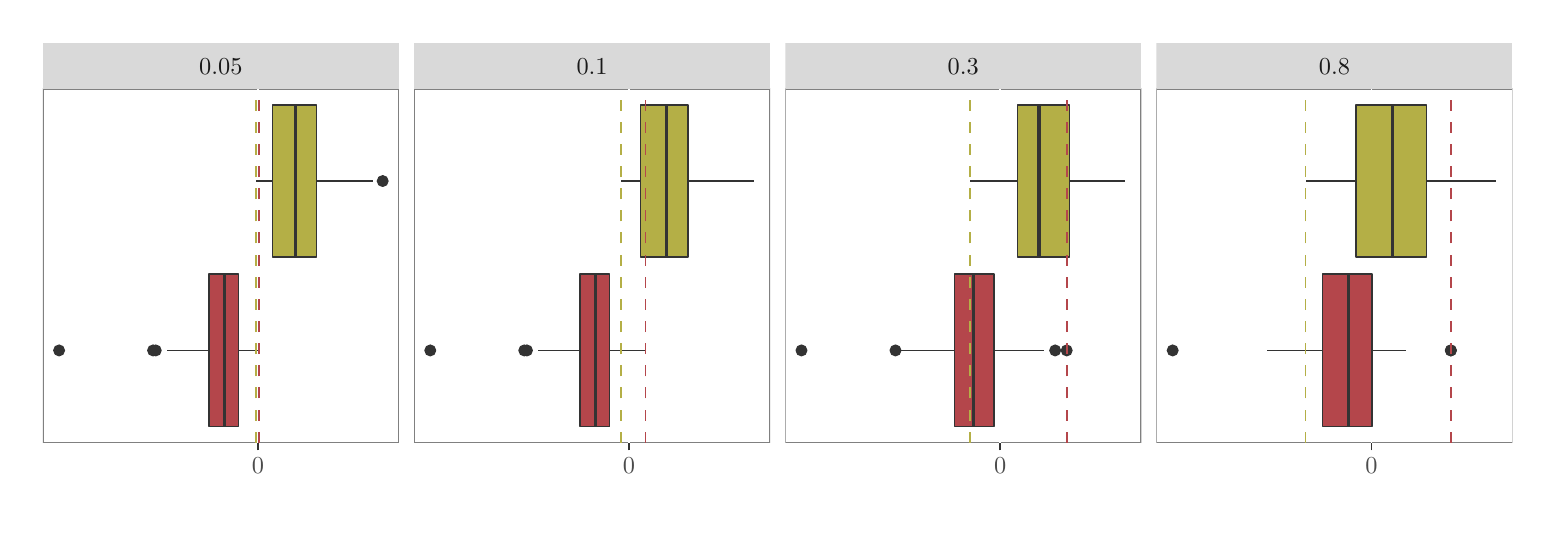
\begin{tikzpicture}[x=1pt,y=1pt]
\definecolor{fillColor}{RGB}{255,255,255}
\path[use as bounding box,fill=fillColor,fill opacity=0.00] (0,0) rectangle (542.02,180.67);
\begin{scope}
\path[clip] (  0.00,  0.00) rectangle (542.02,180.67);
\definecolor{drawColor}{RGB}{255,255,255}
\definecolor{fillColor}{RGB}{255,255,255}

\path[draw=drawColor,line width= 0.6pt,line join=round,line cap=round,fill=fillColor] (  0.00,  0.00) rectangle (542.03,180.68);
\end{scope}
\begin{scope}
\path[clip] (  5.50, 30.69) rectangle (134.13,158.60);
\definecolor{drawColor}{gray}{0.50}
\definecolor{fillColor}{RGB}{255,255,255}

\path[draw=drawColor,line width= 0.6pt,line join=round,line cap=round,fill=fillColor] (  5.50, 30.69) rectangle (134.13,158.60);
\definecolor{drawColor}{RGB}{255,255,255}

\path[draw=drawColor,line width= 0.6pt,line join=round] ( 83.17, 30.69) --
	( 83.17,158.60);
\definecolor{drawColor}{gray}{0.20}
\definecolor{fillColor}{gray}{0.20}

\path[draw=drawColor,line width= 0.4pt,line join=round,line cap=round,fill=fillColor] ( 46.28, 64.04) circle (  1.96);

\path[draw=drawColor,line width= 0.4pt,line join=round,line cap=round,fill=fillColor] ( 11.35, 64.04) circle (  1.96);

\path[draw=drawColor,line width= 0.4pt,line join=round,line cap=round,fill=fillColor] ( 45.31, 64.04) circle (  1.96);

\path[draw=drawColor,line width= 0.6pt,line join=round] ( 76.12, 64.04) -- ( 83.52, 64.04);

\path[draw=drawColor,line width= 0.6pt,line join=round] ( 65.51, 64.04) -- ( 50.29, 64.04);
\definecolor{fillColor}{RGB}{180,70,75}

\path[draw=drawColor,line width= 0.6pt,line join=round,line cap=round,fill=fillColor] ( 76.12, 36.50) --
	( 65.51, 36.50) --
	( 65.51, 91.58) --
	( 76.12, 91.58) --
	( 76.12, 36.50) --
	cycle;

\path[draw=drawColor,line width= 1.1pt,line join=round] ( 71.02, 36.50) -- ( 71.02, 91.58);
\definecolor{fillColor}{gray}{0.20}

\path[draw=drawColor,line width= 0.4pt,line join=round,line cap=round,fill=fillColor] (128.28,125.25) circle (  1.96);

\path[draw=drawColor,line width= 0.6pt,line join=round] (104.40,125.25) -- (124.75,125.25);

\path[draw=drawColor,line width= 0.6pt,line join=round] ( 88.50,125.25) -- ( 82.48,125.25);
\definecolor{fillColor}{RGB}{180,175,70}

\path[draw=drawColor,line width= 0.6pt,line join=round,line cap=round,fill=fillColor] (104.40, 97.70) --
	( 88.50, 97.70) --
	( 88.50,152.79) --
	(104.40,152.79) --
	(104.40, 97.70) --
	cycle;

\path[draw=drawColor,line width= 1.1pt,line join=round] ( 96.63, 97.70) -- ( 96.63,152.79);
\definecolor{drawColor}{RGB}{180,175,70}

\path[draw=drawColor,line width= 0.6pt,dash pattern=on 4pt off 4pt ,line join=round] ( 82.48, 30.69) -- ( 82.48,158.60);
\definecolor{drawColor}{RGB}{180,70,75}

\path[draw=drawColor,line width= 0.6pt,dash pattern=on 4pt off 4pt ,line join=round] ( 83.52, 30.69) -- ( 83.52,158.60);
\end{scope}
\begin{scope}
\path[clip] (139.63, 30.69) rectangle (268.26,158.60);
\definecolor{drawColor}{gray}{0.50}
\definecolor{fillColor}{RGB}{255,255,255}

\path[draw=drawColor,line width= 0.6pt,line join=round,line cap=round,fill=fillColor] (139.63, 30.69) rectangle (268.26,158.60);
\definecolor{drawColor}{RGB}{255,255,255}

\path[draw=drawColor,line width= 0.6pt,line join=round] (217.30, 30.69) --
	(217.30,158.60);
\definecolor{drawColor}{gray}{0.20}
\definecolor{fillColor}{gray}{0.20}

\path[draw=drawColor,line width= 0.4pt,line join=round,line cap=round,fill=fillColor] (180.41, 64.04) circle (  1.96);

\path[draw=drawColor,line width= 0.4pt,line join=round,line cap=round,fill=fillColor] (145.48, 64.04) circle (  1.96);

\path[draw=drawColor,line width= 0.4pt,line join=round,line cap=round,fill=fillColor] (179.44, 64.04) circle (  1.96);

\path[draw=drawColor,line width= 0.6pt,line join=round] (210.25, 64.04) -- (223.25, 64.04);

\path[draw=drawColor,line width= 0.6pt,line join=round] (199.64, 64.04) -- (184.42, 64.04);
\definecolor{fillColor}{RGB}{180,70,75}

\path[draw=drawColor,line width= 0.6pt,line join=round,line cap=round,fill=fillColor] (210.25, 36.50) --
	(199.64, 36.50) --
	(199.64, 91.58) --
	(210.25, 91.58) --
	(210.25, 36.50) --
	cycle;

\path[draw=drawColor,line width= 1.1pt,line join=round] (205.15, 36.50) -- (205.15, 91.58);

\path[draw=drawColor,line width= 0.6pt,line join=round] (238.53,125.25) -- (262.42,125.25);

\path[draw=drawColor,line width= 0.6pt,line join=round] (221.39,125.25) -- (214.37,125.25);
\definecolor{fillColor}{RGB}{180,175,70}

\path[draw=drawColor,line width= 0.6pt,line join=round,line cap=round,fill=fillColor] (238.53, 97.70) --
	(221.39, 97.70) --
	(221.39,152.79) --
	(238.53,152.79) --
	(238.53, 97.70) --
	cycle;

\path[draw=drawColor,line width= 1.1pt,line join=round] (230.76, 97.70) -- (230.76,152.79);
\definecolor{drawColor}{RGB}{180,175,70}

\path[draw=drawColor,line width= 0.6pt,dash pattern=on 4pt off 4pt ,line join=round] (214.37, 30.69) -- (214.37,158.60);
\definecolor{drawColor}{RGB}{180,70,75}

\path[draw=drawColor,line width= 0.6pt,dash pattern=on 4pt off 4pt ,line join=round] (223.25, 30.69) -- (223.25,158.60);
\end{scope}
\begin{scope}
\path[clip] (273.76, 30.69) rectangle (402.39,158.60);
\definecolor{drawColor}{gray}{0.50}
\definecolor{fillColor}{RGB}{255,255,255}

\path[draw=drawColor,line width= 0.6pt,line join=round,line cap=round,fill=fillColor] (273.76, 30.69) rectangle (402.39,158.60);
\definecolor{drawColor}{RGB}{255,255,255}

\path[draw=drawColor,line width= 0.6pt,line join=round] (351.43, 30.69) --
	(351.43,158.60);
\definecolor{drawColor}{gray}{0.20}
\definecolor{fillColor}{gray}{0.20}

\path[draw=drawColor,line width= 0.4pt,line join=round,line cap=round,fill=fillColor] (279.61, 64.04) circle (  1.96);

\path[draw=drawColor,line width= 0.4pt,line join=round,line cap=round,fill=fillColor] (375.45, 64.04) circle (  1.96);

\path[draw=drawColor,line width= 0.4pt,line join=round,line cap=round,fill=fillColor] (313.58, 64.04) circle (  1.96);

\path[draw=drawColor,line width= 0.4pt,line join=round,line cap=round,fill=fillColor] (371.28, 64.04) circle (  1.96);

\path[draw=drawColor,line width= 0.6pt,line join=round] (349.06, 64.04) -- (367.41, 64.04);

\path[draw=drawColor,line width= 0.6pt,line join=round] (334.94, 64.04) -- (314.54, 64.04);
\definecolor{fillColor}{RGB}{180,70,75}

\path[draw=drawColor,line width= 0.6pt,line join=round,line cap=round,fill=fillColor] (349.06, 36.50) --
	(334.94, 36.50) --
	(334.94, 91.58) --
	(349.06, 91.58) --
	(349.06, 36.50) --
	cycle;

\path[draw=drawColor,line width= 1.1pt,line join=round] (341.67, 36.50) -- (341.67, 91.58);

\path[draw=drawColor,line width= 0.6pt,line join=round] (376.45,125.25) -- (396.55,125.25);

\path[draw=drawColor,line width= 0.6pt,line join=round] (357.68,125.25) -- (340.54,125.25);
\definecolor{fillColor}{RGB}{180,175,70}

\path[draw=drawColor,line width= 0.6pt,line join=round,line cap=round,fill=fillColor] (376.45, 97.70) --
	(357.68, 97.70) --
	(357.68,152.79) --
	(376.45,152.79) --
	(376.45, 97.70) --
	cycle;

\path[draw=drawColor,line width= 1.1pt,line join=round] (365.44, 97.70) -- (365.44,152.79);
\definecolor{drawColor}{RGB}{180,175,70}

\path[draw=drawColor,line width= 0.6pt,dash pattern=on 4pt off 4pt ,line join=round] (340.54, 30.69) -- (340.54,158.60);
\definecolor{drawColor}{RGB}{180,70,75}

\path[draw=drawColor,line width= 0.6pt,dash pattern=on 4pt off 4pt ,line join=round] (375.45, 30.69) -- (375.45,158.60);
\end{scope}
\begin{scope}
\path[clip] (407.89, 30.69) rectangle (536.52,158.60);
\definecolor{drawColor}{gray}{0.50}
\definecolor{fillColor}{RGB}{255,255,255}

\path[draw=drawColor,line width= 0.6pt,line join=round,line cap=round,fill=fillColor] (407.89, 30.69) rectangle (536.52,158.60);
\definecolor{drawColor}{RGB}{255,255,255}

\path[draw=drawColor,line width= 0.6pt,line join=round] (485.56, 30.69) --
	(485.56,158.60);
\definecolor{drawColor}{gray}{0.20}
\definecolor{fillColor}{gray}{0.20}

\path[draw=drawColor,line width= 0.4pt,line join=round,line cap=round,fill=fillColor] (413.74, 64.04) circle (  1.96);

\path[draw=drawColor,line width= 0.4pt,line join=round,line cap=round,fill=fillColor] (514.21, 64.04) circle (  1.96);

\path[draw=drawColor,line width= 0.4pt,line join=round,line cap=round,fill=fillColor] (514.30, 64.04) circle (  1.96);

\path[draw=drawColor,line width= 0.6pt,line join=round] (485.70, 64.04) -- (498.11, 64.04);

\path[draw=drawColor,line width= 0.6pt,line join=round] (467.90, 64.04) -- (447.71, 64.04);
\definecolor{fillColor}{RGB}{180,70,75}

\path[draw=drawColor,line width= 0.6pt,line join=round,line cap=round,fill=fillColor] (485.70, 36.50) --
	(467.90, 36.50) --
	(467.90, 91.58) --
	(485.70, 91.58) --
	(485.70, 36.50) --
	cycle;

\path[draw=drawColor,line width= 1.1pt,line join=round] (477.13, 36.50) -- (477.13, 91.58);

\path[draw=drawColor,line width= 0.6pt,line join=round] (505.47,125.25) -- (530.68,125.25);

\path[draw=drawColor,line width= 0.6pt,line join=round] (480.07,125.25) -- (461.77,125.25);
\definecolor{fillColor}{RGB}{180,175,70}

\path[draw=drawColor,line width= 0.6pt,line join=round,line cap=round,fill=fillColor] (505.47, 97.70) --
	(480.07, 97.70) --
	(480.07,152.79) --
	(505.47,152.79) --
	(505.47, 97.70) --
	cycle;

\path[draw=drawColor,line width= 1.1pt,line join=round] (493.27, 97.70) -- (493.27,152.79);
\definecolor{drawColor}{RGB}{180,175,70}

\path[draw=drawColor,line width= 0.6pt,dash pattern=on 4pt off 4pt ,line join=round] (461.77, 30.69) -- (461.77,158.60);
\definecolor{drawColor}{RGB}{180,70,75}

\path[draw=drawColor,line width= 0.6pt,dash pattern=on 4pt off 4pt ,line join=round] (514.30, 30.69) -- (514.30,158.60);
\end{scope}
\begin{scope}
\path[clip] (  5.50,158.60) rectangle (134.13,175.17);
\definecolor{fillColor}{gray}{0.85}

\path[fill=fillColor] (  5.50,158.60) rectangle (134.13,175.18);
\definecolor{drawColor}{gray}{0.10}

\node[text=drawColor,anchor=base,inner sep=0pt, outer sep=0pt, scale=  0.88] at ( 69.82,163.86) {0.05};
\end{scope}
\begin{scope}
\path[clip] (139.63,158.60) rectangle (268.26,175.17);
\definecolor{fillColor}{gray}{0.85}

\path[fill=fillColor] (139.63,158.60) rectangle (268.26,175.18);
\definecolor{drawColor}{gray}{0.10}

\node[text=drawColor,anchor=base,inner sep=0pt, outer sep=0pt, scale=  0.88] at (203.95,163.86) {0.1};
\end{scope}
\begin{scope}
\path[clip] (273.76,158.60) rectangle (402.39,175.17);
\definecolor{fillColor}{gray}{0.85}

\path[fill=fillColor] (273.76,158.60) rectangle (402.39,175.18);
\definecolor{drawColor}{gray}{0.10}

\node[text=drawColor,anchor=base,inner sep=0pt, outer sep=0pt, scale=  0.88] at (338.08,163.86) {0.3};
\end{scope}
\begin{scope}
\path[clip] (407.89,158.60) rectangle (536.52,175.17);
\definecolor{fillColor}{gray}{0.85}

\path[fill=fillColor] (407.89,158.60) rectangle (536.52,175.18);
\definecolor{drawColor}{gray}{0.10}

\node[text=drawColor,anchor=base,inner sep=0pt, outer sep=0pt, scale=  0.88] at (472.21,163.86) {0.8};
\end{scope}
\begin{scope}
\path[clip] (  0.00,  0.00) rectangle (542.02,180.67);
\definecolor{drawColor}{gray}{0.20}

\path[draw=drawColor,line width= 0.6pt,line join=round] ( 83.17, 27.94) --
	( 83.17, 30.69);
\end{scope}
\begin{scope}
\path[clip] (  0.00,  0.00) rectangle (542.02,180.67);
\definecolor{drawColor}{gray}{0.30}

\node[text=drawColor,anchor=base,inner sep=0pt, outer sep=0pt, scale=  0.88] at ( 83.17, 19.68) {0};
\end{scope}
\begin{scope}
\path[clip] (  0.00,  0.00) rectangle (542.02,180.67);
\definecolor{drawColor}{gray}{0.20}

\path[draw=drawColor,line width= 0.6pt,line join=round] (217.30, 27.94) --
	(217.30, 30.69);
\end{scope}
\begin{scope}
\path[clip] (  0.00,  0.00) rectangle (542.02,180.67);
\definecolor{drawColor}{gray}{0.30}

\node[text=drawColor,anchor=base,inner sep=0pt, outer sep=0pt, scale=  0.88] at (217.30, 19.68) {0};
\end{scope}
\begin{scope}
\path[clip] (  0.00,  0.00) rectangle (542.02,180.67);
\definecolor{drawColor}{gray}{0.20}

\path[draw=drawColor,line width= 0.6pt,line join=round] (351.43, 27.94) --
	(351.43, 30.69);
\end{scope}
\begin{scope}
\path[clip] (  0.00,  0.00) rectangle (542.02,180.67);
\definecolor{drawColor}{gray}{0.30}

\node[text=drawColor,anchor=base,inner sep=0pt, outer sep=0pt, scale=  0.88] at (351.43, 19.68) {0};
\end{scope}
\begin{scope}
\path[clip] (  0.00,  0.00) rectangle (542.02,180.67);
\definecolor{drawColor}{gray}{0.20}

\path[draw=drawColor,line width= 0.6pt,line join=round] (485.56, 27.94) --
	(485.56, 30.69);
\end{scope}
\begin{scope}
\path[clip] (  0.00,  0.00) rectangle (542.02,180.67);
\definecolor{drawColor}{gray}{0.30}

\node[text=drawColor,anchor=base,inner sep=0pt, outer sep=0pt, scale=  0.88] at (485.56, 19.68) {0};
\end{scope}
\end{tikzpicture}
